\documentclass{article}

% Language setting
% Replace `english' with e.g. `spanish' to change the document language
\usepackage[english]{babel}

% Set page size and margins
% Replace `letterpaper' with `a4paper' for UK/EU standard size
\usepackage[letterpaper,top=2cm,bottom=2cm,left=3cm,right=3cm,marginparwidth=1.75cm]{geometry}

% Useful packages
\usepackage{amsmath}
\usepackage{amsfonts}
\usepackage{graphicx}
\usepackage{xcolor}
\usepackage{booktabs}
\usepackage{hyperref}

\usepackage[labelformat=simple]{subcaption}
\renewcommand\thesubfigure{(\alph{subfigure})}
\usepackage[font=small,labelfont=bf]{caption}
\allowdisplaybreaks

\usepackage{tikz}
\usetikzlibrary{automata, positioning, arrows}

\tikzset{
    ->,                                         % makes the edges directed
    >=stealth,                                  % makes the arrow heads bold
    node distance=3cm,                          % specifies the minimum distance between two nodes. Change if necessary.
   % every state/.style={},                 % sets the properties for each ’state’ node
    initial text=$ $,                       % sets the text that appears on the start arrow
}

\newcommand{\sil}{\langle sil \rangle}
\newcommand{\blank}{\langle b \rangle}

\title{WFST formulation of lattice-free MMI}
\author{Desh Raj, Matthew Wiesner}

\begin{document}
\maketitle

\begin{abstract}
We derive the lattice-free maximum mutual information (LF-MMI) based ASR model from first principles of WFSTs. 
%
This leads to discussion of implementation variants such as end-to-end LF-MMI and the \texttt{icefall} MMI. 
%
We also present its connection to the popular CTC objective. 
\end{abstract}

\section{What is an ASR ``model''?}
\label{sec:asr}

Suppose we have a speech input $\mathbf{X}\in \mathbb{R}^{T^{\prime}\times F}$. 
%
We have some reference transcript $\mathbf{w} = (w_1,\ldots,w_L)$, where $w_l \in \Sigma$, and $\Sigma$ is the vocabulary. 
%
The goal of ASR is to predict $\hat{\mathbf{w}}$, which is the best estimate for $\mathbf{w}$. 
%
This is usually done by modeling $P(\mathbf{w}|\mathbf{X})$ (either directly or indirectly using Bayes rule) and computing the Bayes optimal solution (exact or approximate), i.e., 

\begin{equation}
\label{eq:asr}
    \hat{\mathbf{w}} = \text{arg}\max_{\mathbf{w}} P(\mathbf{w}|\mathbf{X})
\end{equation}

\paragraph{} Most complications in the ASR task arise from the fact that $T'$ is not equal to $L$, and there is no known alignment between the input and output sequence. 
%
Indeed, if an alignment is known, we could simply use frame-level cross-entropy for training, as was standard in older hybrid models before sequence-level objectives became popular.

\paragraph{} When we talk about ASR ``models,'' we are usually referring to a framework comprising several components, which we will discuss next.

\subsection{Frame-synchronous and label-synchronous models}

Based on how the input is processed, ASR models can be categorized as frame-synchronous or label-synchronous~\cite{Prabhavalkar2017ACO, Dong2020ACO}. 
%
Frame-synchronous models are driven by the input frames: they process the frames one-at-a-time and stop when there are no more frames to process. 
%
Some examples are traditional HMM-based models, CTC, RNN-transducers, etc. Label-synchronous models, on the other hand, are driven by the output text. 
%
Often they process the entire input and then start predicting output tokens one-by-one until an \texttt{<eos>} token is predicted. 
%
The dominant label-synchronous model is the attention-based encoder-decoder. 
%
In this document, our focus is on frame-synchronous models since they have several obvious advantages:

\begin{enumerate}
    \item They are naturally streaming if the encoder is left-context only.
    \item In addition to the tokens, they provide a sense of ``alignment'' between the label and the frames, which can be used to estimate token-level timestamps.
\end{enumerate}

\subsection{Network architecture}

Modern ASR systems usually process the input $\mathbf{X}$ using a neural network function $h(\mathbf{X}) = \mathbf{h} \in \mathbb{R}^{T\times D}$, where $T \leq T'$ usually due to frame sub-sampling, and so equation (\ref{eq:asr}) becomes
%
\begin{equation}
    \hat{\mathbf{w}} = \text{arg}\max_{\mathbf{w}} P(\mathbf{w}|\mathbf{h}).
\end{equation}

Here, $h(\cdot)$ may be the functional equivalent of any standard architecture, such as convolutional, recurrent, or self-attention layers. 
%
Often, the encoder architecture itself may also be referred to as the ``model'' by some abuse of notation. 
%
For the purpose of this document, the specific choice of architecture is not important.

\paragraph{} In some cases, the output label sequence may also be processed by a neural network to provide additional context and make the outputs conditionally dependent, such as in RNN-Transducers through a prediction network. 
%
However, this is beyond the scope for this document.

\subsection{Modeling units}

The final transcript that we want to generate using an ASR system would usually contain words. 
%
However, it is often computationally easier for the model to predict the output in the form of sub-words units. 
%
The most common modeling units used are as follows:

\begin{enumerate}
    \item Characters
    \item Phonemes
    \item Character groups, such as bi-chars, tri-chars, etc.
    \item Phoneme groups, such as bi-phones, tri-phones, etc.
    \item Chenones/senones, which are context dependent char/phoneme groups tied with a decision tree
    \item BPE units
\end{enumerate}

\paragraph{} Due to historical reasons (e.g., where the models were developed), CTC models developed using character/BPE units while LF-MMI used senones. 
%
But the choice of modeling unit is not tied to the model, and different units may be used based on their advantages/disadvantages~\cite{zhang_lattice-free_2021}. 
%
For example, using phone-based modeling units requires a phonetic lexicon, and using chenones/senones would require state tying using likelihoods from a GMM. 
%
Modern ``end-to-end'' ASR models have converged to the choice of BPE as the modeling units.

\paragraph{} Nevertheless, in the WFST-based decoding framework, the decoding graph can be built to directly output words even if the model predicts sub-word units. 
%
This is done by composing the graph with the lexicon FST $L$.


\subsection{Label topology}

Earlier, we mentioned that usually when training ASR models, the exact ``alignment'' between $\mathbf{X}$ and $\mathbf{y}$ is not known. 
%
The label topology is the component which defines the mapping between the label sequence and the modeling units. 
%
Let us denote this as $\mathcal{T}$. 
%
Consider also the linear FST denoting the label sequence as $\mathcal{Y}(\mathbf{w})$\footnote{We assume here that $\mathbf{w}$ has been tokenized into the desired modeling units.}. 
%
Then, the ``alignment lattice,'' i.e., the set of all possible alignments mapping to $\mathbf{w}$ is given by the composition of $\mathcal{T}$ and $\mathcal{Y}(\mathbf{w})$, i.e.,

\begin{equation}
    \mathcal{A}(\mathbf{w}) = \mathcal{T} \circ \mathcal{Y}(\mathbf{w}).
\end{equation}

Suppose our vocabulary consists of the characters $a$ and $b$. 
%
For traditional HMM-based systems which also modeled $\sil$ explicitly, a 1-state HMM topology can be represented by Fig.~\ref{fig:hmm_topo}.

\begin{figure}[t]
\begin{subfigure}{0.45\linewidth}
\centering
\resizebox{\textwidth}{!}{%
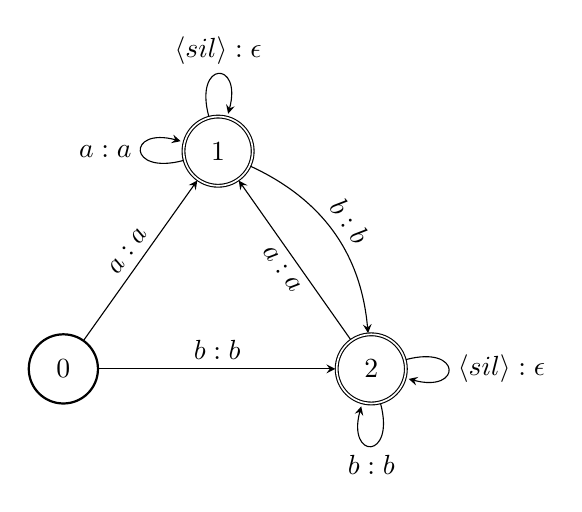
\begin{tikzpicture}

\node[state, style=thick] (q0) {$0$};
\node[state, above right=of q0, xshift=-0.8cm, accepting] (q1) {$1$};
\node[state, right=of q0, accepting] (q2) {$2$};

\draw 
(q1) edge[loop above] node{$\sil:\epsilon$} ()
(q1) edge[loop left] node{$a:a$} ()
(q2) edge[loop right] node{$\sil:\epsilon$} ()
(q2) edge[loop below] node{$b:b$} ()
(q0) edge[sloped, above] node{$a:a$} (q1)
(q1) edge[sloped, above, bend left] node{$b:b$} (q2)
(q2) edge[sloped, below] node{$a:a$} (q1)
(q0) edge[sloped, above] node{$b:b$} (q2);

\end{tikzpicture}
}
\caption{1-state HMM topology}
\label{fig:hmm_topo}
\end{subfigure}
\begin{subfigure}{0.55\linewidth}
\centering
\resizebox{\textwidth}{!}{%
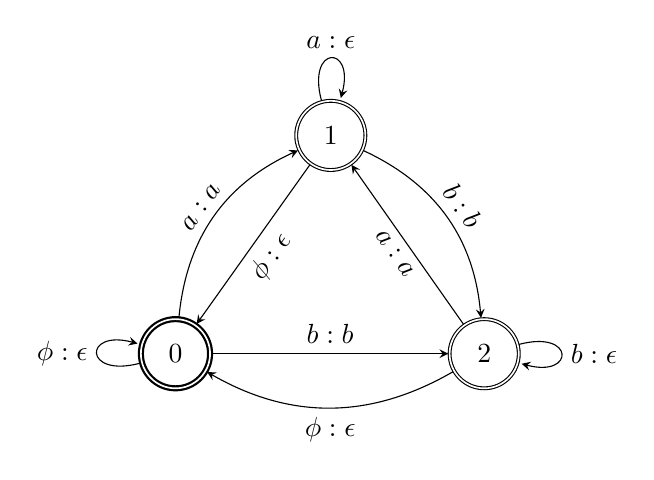
\begin{tikzpicture}

\node[state, style=thick, accepting] (q0) {$0$};
\node[state, above right=of q0, xshift=-0.8cm, accepting] (q1) {$1$};
\node[state, right=of q0, accepting] (q2) {$2$};

\draw 
(q0) edge[loop left] node{$\phi:\epsilon$} ()
(q1) edge[loop above] node{$a:\epsilon$} ()
(q2) edge[loop right] node{$b:\epsilon$} ()
(q0) edge[sloped, above, bend left] node{$a:a$} (q1)
(q1) edge[sloped, below] node{$\phi:\epsilon$} (q0)
(q1) edge[sloped, above, bend left] node{$b:b$} (q2)
(q2) edge[sloped, below] node{$a:a$} (q1)
(q2) edge[sloped, below, bend left] node{$\phi:\epsilon$} (q0)
(q0) edge[sloped, above] node{$b:b$} (q2);

\end{tikzpicture}
}
\caption{CTC topology}
\label{fig:ctc_topo}
\end{subfigure}
\caption{Topology FSTs for standard 1-state HMM and CTC.}
\end{figure}

\paragraph{} Another popular topology in modern ASR systems is the CTC topology. 
%
The CTC topology generates alignments formed by repeating the characters and inserting blanks ($\phi$) to allow repeated characters in the label sequence. 
%
This is shown in Fig.~\ref{fig:ctc_topo}.

\subsection{Training objective}

Let $\mathcal{B}$ denote the many-to-one mapping from an alignment $\mathbf{a}$ to an output label sequence $\mathbf{w}$, which is determined by the topology $\mathcal{T}$ and the input length $T$. Then, we can expand equation (\ref{eq:asr}) using the following:

\begin{equation}
    P(\mathbf{w}|\mathbf{X}) = \sum_{\mathbf{a}\in \mathcal{B}^{-1}(\mathbf{w})} P(\mathbf{a}|\mathbf{X}).
\end{equation}

For discriminative training of the ASR model, we usually maximize the log, i.e.,

\begin{equation}
    \mathcal{L}_{\theta} = \log \left( \sum_{\mathbf{a}\in \mathcal{B}^{-1}(\mathbf{w})} P_{\theta}(\mathbf{a}|\mathbf{X}) \right).
\end{equation}

In a very general setting, the distribution can be written as:

\begin{equation}
    P_{\theta}(\mathbf{a}|\mathbf{X}) = \frac{p(\mathbf{a})\exp(f_{\theta}(\mathbf{X},\mathbf{a}))}{\mathbb{E}_{p(\mathbf{a'})}[\exp(f_{\theta}(\mathbf{X},\mathbf{a'}))]}.
\end{equation}

You may recognize that this as similar to Bayes rule on $P_{\theta}(\mathbf{a}|\mathbf{X})$, where the likelihood is replaced with a general ``potential function'' and the normalization term in the denominator is written using an expectation over all possible alignments. This way of expressing a distribution from raw (un-normalized) scores goes by many names including the Boltzmann, and Gibbs distributions. Finally, the loss function becomes:

\begin{equation}
\label{eq:loss}
    \mathcal{L}_{\theta} = \log \left( \frac{\sum_{\mathbf{a}\in \mathcal{B}^{-1}(\mathbf{w})} p(\mathbf{a})\exp(f_{\theta}(\mathbf{X},\mathbf{a}))}{\mathbb{E}_{p(\mathbf{a'})}[\exp(f_{\theta}(\mathbf{X},\mathbf{a'}))]} \right).
\end{equation}


\section{WFST formulation of LF-MMI}
\label{sec:lfmmi}

Let us now formulate the original LF-MMI objective using the general components described in Section~\ref{sec:asr}. 

\paragraph{} First, we define the following WFSTs on the log-semiring.

\begin{itemize}
\item $H$: This is a 1-state HMM topology~\footnote{In the original paper~\cite{Povey2016PurelySN}, the 2-state skip HMM topology was used, but it was later simplified to the 1-state HMM topology.}.
\item $\phi$: This is the ``sausage'' lattice representing the output of the neural network encoder. It is equivalent to a $T \times |\Sigma|$ matrix where each cell $(t,s)$ contains the score for token $s$ at time $t$.
\item $G$: This is the WFST representation of the language model over the modeling units.
\end{itemize}

\paragraph{} We create 2 versions of the decoding graph:

\begin{enumerate}
    \item \textit{Numerator graph} ($M_N$): $H \circ \mathcal{Y}(\mathbf{w}) \circ G$ 
    \item \textit{Denominator graph} ($M_D$): $H \circ G$
\end{enumerate}

It is evident that the numerator graph is just a \textit{clamped} version of the general decoding graph, where the clamping is with respect to the target sequence $\mathbf{w}$.

\paragraph{} Let us now re-write equation~(\ref{eq:loss}).
\begin{align}
\mathcal{L}_{\theta} &= \log \left( \frac{\sum_{\mathbf{a}\in \mathcal{B}^{-1}(\mathbf{w})} p(\mathbf{a})\exp(f_{\theta}(\mathbf{X},\mathbf{a}))}{\mathbb{E}_{p(\mathbf{a'})}[\exp(f_{\theta}(\mathbf{X},\mathbf{a'}))]} \right) \\
&= \log \left( \sum_{\mathbf{a}\in \mathcal{B}^{-1}(\mathbf{w})} p(\mathbf{a})\exp(f_{\theta}(\mathbf{X},\mathbf{a})) \right) - \log \mathbb{E}_{p(\mathbf{a'})}[\exp(f_{\theta}(\mathbf{X},\mathbf{a'}))] \\
&=  \underbrace{\left[[ \phi \circ M_N \right]]}_{\text{numerator lattice}} - \underbrace{\left[[ \phi \circ M_D \right]]}_{\text{denominator lattice}}, \label{eq:WFST_MMI}
\end{align}
where $[[\cdot]]$ denotes the forward score on the WFST.

\paragraph{} This is because the WFSTs are already defined over the log semiring. The potential functions are obtained from the arc weights on $\phi$. For the numerator term, the ``clamping'' (composition with $\mathcal{Y}(\mathbf{w})$) is equivalent to summing over the subset $\mathcal{B}^{-1}(\mathbf{w})$.

\subsection{Gradient}
% Show how to compute gradients in this frameworks
\paragraph{} To train models using this objective, we need to compute gradients w.r.t. the neural network outputs $\phi$. We will show how these gradients can also be computed via dynamic programming, i.e., using WFST operations on the numerator and denominator lattices. By denominator / numerator lattice (as opposed to graph), we mean the two terms in Equation \ref{eq:WFST_MMI}.

The forward pass for an input $\mathbf{X}$ can be expressed as
\begin{equation}
    [\![\phi \circ M]\!] = \log{\sum_{\mathbf{a} \in M} p\left(\mathbf{a}\right)e^{\sum_{t=0}^{T-1}\phi_{\mathbf{a}_t}^t }}
\end{equation}

Note that in this case $f_\theta\left(\mathbf{X}, \mathbf{a}\right) = \sum_{t=0}^{T-1}\phi_{\mathbf{a}_t}^t$, is the score of alignment, $\mathbf{a}$, occurring with input, $\mathbf{X}$. In other words, the score of the alignment is the sum of scores of each individual symbol in the sequence. We will see this again in Section \ref{sec:ctc}.

We derive the gradient for this objective function below. 
\begin{align}
    \nabla_{\phi_{i}^\tau} \log{ p_\theta\left(\mathbf{w} | \mathbf{X}\right)} &= \nabla_{\phi_{i}^\tau} [\![\phi \circ M_N]\!] - \nabla_{\phi_{i}^\tau} [\![\phi \circ M_D]\!] \\
    = \frac{\sum_{\mathbf{a} \in M_N} p\left(\mathbf{a}\right)e^{\sum_{t=0}^{T-1}\phi_{\mathbf{a}_t}^t} \sum_{t=0}^{T-1}\nabla_{\phi_{i}^\tau} \phi_{\mathbf{a}_t}^t}{\sum_{\mathbf{a}^\prime \in M_{N}} p\left(\mathbf{a}^\prime\right)e^{\sum_{t=0}^{T-1}\phi_{\mathbf{a}^\prime_t}^t}} &- \frac{\sum_{\mathbf{a} \in M_D} p\left(\mathbf{a}\right)e^{\sum_{t=0}^{T-1}\phi_{\mathbf{a}_t}^t} \sum_{t=0}^{T-1}\nabla_{\phi_{i}^\tau} \phi_{\mathbf{a}_t}^t}{\sum_{\mathbf{a}^\prime \in M_D} p\left(\mathbf{a}^\prime\right)e^{\sum_{t=0}^{T-1}\phi_{\mathbf{a}^\prime_t}^t}} \\
    = \frac{\sum_{\mathbf{a} \in M_N} p\left(\mathbf{a}\right)e^{\sum_{t=0}^{T-1}\phi_{\mathbf{a}_t}^t} \mathbb{I}\left(\mathbf{a}_\tau, i\right)}{\sum_{\mathbf{a}^\prime \in M_N} p\left(\mathbf{a}^\prime\right)e^{\sum_{t=0}^{T-1}\phi_{\mathbf{a}^\prime_t}^t}} &- \frac{\sum_{\mathbf{a} \in M_D} p\left(\mathbf{a}\right)e^{\sum_{t=0}^{T-1}\phi_{\mathbf{a}_t}^t} \mathbb{I}\left(\mathbf{a}_\tau, i\right)}{\sum_{\mathbf{a}^\prime \in M_D} p\left(\mathbf{a}^\prime\right)e^{\sum_{t=0}^{T-1}\phi_{\mathbf{a}^\prime_t}^t}} \\
    = \sum_{\mathbf{a} \in M_N} p\left(\mathbf{a} | \mathbf{X}, \mathbf{w}\right)\mathbb{I}\left(\mathbf{a}_\tau, i\right) &- \sum_{\mathbf{a} \in M_D} p\left(\mathbf{a} | \mathbf{X}\right)\mathbb{I}\left(\mathbf{a}_\tau, i\right).
\end{align}

Let $l\left[\mathbf{a}_\tau\right]$ indicate the label on arc $\mathbf{a}_\tau$. In the above equations $\mathbb{I}\left(\mathbf{a}_\tau, i\right)$ is the indicator function.

\begin{equation*}
\mathbb{I}\left(\mathbf{a}_\tau, i\right) =
\begin{cases} 1 & l\left[\mathbf{a}_\tau\right] = i \\ 0 & l\left[\mathbf{a}_\tau\right] \neq i \end{cases}
\end{equation*}

We see then that the gradient is just a difference between the soft-counts in the numerator and denominator graphs of arcs with label, $l\left[\mathbf{a}_\tau\right]$, equal to $i$, occurring at time $\tau$. These quantities can be efficiently computed by running the forward and backward algorithm on the lattices produced by $\phi \circ M_D$/$M_N$ and computing the forward and backward scores $a_{M_D}\left(s, \tau\right), b_{M_D}\left(s, \tau\right), a_{M_N}\left(s, \tau\right),b_{M_N}\left(s, \tau\right)$. Note that we overloaded notation a little here when we are referring to forward and backward scores on the lattices, $\phi \circ M_{\{N,D\}}$ by simply writing $M_{\{N,D\}}$. The terms in the gradient can be expressed in terms of these quantities. $s$ refers to a particular state in the WFST, Let $L\left(\mathbf{a}_\tau\right), R\left(\mathbf{a}_\tau\right)$, be the states from which an arc, $\mathbf{a}_\tau$ leaves and into which it enters respectively, and let $w_M\left(\mathbf{a}_\tau\right)$ be the weight on that arc in the lattice $\phi \circ M$. Then the sum of all paths taking arc, $\mathbf{a}_\tau$, which we will define as $c\left(\mathbf{a}_\tau\right)$, can be expressed as 

\begin{equation}
    c_M\left(\mathbf{a}_\tau\right) = a_{M}\left(L\left(\mathbf{a}_\tau\right), \tau\right)w_M\left(\mathbf{a}_\tau\right) b_{M}\left(R\left(\mathbf{a}_\tau\right), \tau\right).
\end{equation}

Finally, the gradient can be computed by re-using the forward scores (you can think of them as normalizers so that $c_M\left(\cdot\right)$ is a soft-count, and not just an arbitrary score) as

\begin{align}
     \nabla_{\phi_{i}^\tau}\log{ p_\theta\left(\mathbf{w} | \mathbf{x}\right)} &= \sum_{\mathbf{a}_\tau \in M_N : l\left[\mathbf{a}_\tau\right] = i}\frac{c_{M_N}\left(\mathbf{a}_\tau\right)}{[\![\phi \circ M_N]\!]} - \sum_{\mathbf{a}_\tau \in M_D : l\left[\mathbf{a}_\tau\right] = i}\frac{c_{M_D}\left(\mathbf{a}_\tau\right)}{[\![\phi \circ M_D]\!]}.
\end{align}

Therefore, the objective and gradient of MMI type objectives can be computed by WFST operations on appropriately defined graphs. This formulation is general and only relied on a single assumption -- that $f_\theta\left(\mathbf{X}, \mathbf{a}\right) = \sum_{t=0}^{T-1}\phi_{\mathbf{a}_t}^t$, be the score of alignment, $\mathbf{a}$, occurring with input $\mathbf{X}$. When we interpret $\phi_{\mathbf{a}_t}^t$ as log-probabilities, this is equivalent to saying that the probability of the next symbol, $\mathbf{a}_t$ in alignment $\mathbf{a}$ is conditionally independent of its history given input $\mathbf{X}$. This is the Markov assumption and is what enables representing this type of objective using WFSTs.


\section{Different LF-MMI implementations}

Different choices for the model components result in different existing implementations of the LF-MMI model. For all of these, the training objective remains the same; the difference lies merely in the choice of architecture, modeling unit, or label topology. We summarize some of these implementations in the following table.

\begin{table}[h]
\centering
\caption{Different LF-MMI implementations}
\label{tab:variants}
\begin{tabular}{@{}llll@{}}
\toprule
\textbf{Component} & \textbf{Kaldi (original)}~\cite{Povey2016PurelySN} & \textbf{Kaldi (E2E)}~\cite{hadian_end--end_2018} & \textbf{Icefall}$^{\dagger}$ \\ \midrule
Encoder & TDNN & TDNN-LSTM & Conformer \\
Modeling unit & Senones & Full bi-phones & BPE \\
Label topology & 2-state skip HMM (acyclic) & 2-state skip HMM, 1-state HMM & CTC \\
G.fst & 4-gram phone LM & 4-gram phone LM & 2-gram BPE LM \\ \bottomrule
\multicolumn{4}{@{}l}{$^{\dagger}$\footnotesize{\url{https://github.com/k2-fsa/icefall/blob/master/icefall/mmi.py}}} \\
\end{tabular}
\end{table}

\section{WFST formulation of CTC}
\label{sec:ctc}
Let us quickly see how the popular CTC model can be formulated as a special case of the general MMI training. For this, we take equation~(\ref{eq:loss}) and specialize it as follows:

\begin{itemize}
    \item $\mathcal{B}$ is set as the mapping generated by the CTC topology.
    \item $p(\mathbf{a})$ is set as the uniform distribution.
    \item $f_{\theta}(\mathbf{X},\mathbf{a}) = \sum_t \phi_{a_t}^t$, i.e., the score of an alignment $\mathbf{a}$ is set as the sum of its path weights in the sausage lattice $\phi$.
\end{itemize}

With these assignments, we can simplify equation~(\ref{eq:loss}) as follows.

\begin{align}
\mathcal{L}_{\theta} &= \log \left( \frac{\sum_{\mathbf{a}\in \mathcal{B}^{-1}(\mathbf{w})} p(\mathbf{a})\exp(f_{\theta}(\mathbf{X},\mathbf{a}))}{\mathbb{E}_{p(\mathbf{a'})}[\exp(f_{\theta}(\mathbf{X},\mathbf{a'}))]} \right) \\
&= \log \sum_{\mathbf{a}\in \mathcal{B}^{-1}(\mathbf{w})} \left( \frac{ \exp(\sum_t \phi_{a_t}^t)}{\sum_{\mathbf{a}^{\prime}} \exp(\sum_t \phi_{a_t^{\prime}}^t)} \right) \\
&= \log \sum_{\mathbf{a}\in \mathcal{B}^{-1}(\mathbf{w})} \left( \frac{\prod_t \exp(\phi_{a_t}^t)}{\sum_{\mathbf{a}^{\prime}} \prod_t \exp(\phi_{a_t^{\prime}}^t)} \right) \\
&= \log \sum_{\mathbf{a}\in \mathcal{B}^{-1}(\mathbf{w})} \left( \frac{\prod_t \exp(\phi_{a_t}^t)}{\prod_t \sum_{\mathbf{a}^{\prime}_t} \exp(\phi_{a_t^{\prime}}^t)} \right) \label{eq:trick} \\
&= \log \sum_{\mathbf{a}\in \mathcal{B}^{-1}(\mathbf{w})} \prod_t \underbrace{\frac{\exp(\phi_{a_t}^t)}{\sum_{\mathbf{a}_t^{\prime}}\exp(\phi_{a_t^{\prime}}^t)}}_{\text{locally normalized scores}} \\
&= \log \sum_{\mathbf{a}\in \mathcal{B}^{-1}(\mathbf{w})} \prod_t p_{\theta}(a_t|\mathbf{X}) \\
&= \log \sum_{\mathbf{a}\in \mathcal{B}^{-1}(\mathbf{w})} P(\mathbf{a}|\mathbf{X}).
\end{align}

\paragraph{} The important step here is the trick in equation~(\ref{eq:trick}), which only holds because of the conditional independence assumption in CTC.

\paragraph{} Therefore, we can compute the CTC objective and its gradients similar to MMI, by locally normalizing $\phi$ (using softmax) and then using the same WFST computations but without the denominator term.

\bibliographystyle{abbrv}
\bibliography{refs}

\end{document}